\documentclass[a4paper,10pt]{article}
%\usepackage[latin1]{inputenc} % Paquetes de idioma
\usepackage[utf8]{inputenc} % Paquetes de idioma (Este encoding toma acentos :) )
\usepackage[spanish]{babel} % Paquetes de idioma
\usepackage{graphicx} % Paquete para ingresar gráficos
\usepackage{grffile}
\usepackage{hyperref}
\usepackage{fancybox}
\usepackage{amsmath}
\usepackage{amsfonts}
\usepackage{listings}
\usepackage{float}
% Paquetes de macros de Circuitos
%\usepackage{pstricks}
\usepackage{tikz}

% Encabezado y Pié de página
\usepackage{fancyhdr} % Paquete para encabezados y pie de página
\pagestyle{fancy} % Sin esta línea no se imprimiría el encabezado en todas las páginas

\fancyhf{} %  Borra el encabezado anterior (Por defecto escribe el títutlo de la sección en la que se encuentra la hoja
\setlength{\headheight}{22.55pt}
\fancyhead[L]{
	{\textsf{Facultad de Ingenier\'ia $-$ Universidad de Buenos Aires \\ 66.44 Instrumentos Electrónicos}}
}
%\addtocounter{page}{5}
\fancyhead[R]{\thepage}

\renewcommand{\footrulewidth}{0.4pt} % Ajusta el tamaño de las líneas separadoras en el pié de página
\renewcommand{\headrulewidth}{0.4pt} % Ajusta el tamaño de las líneas separadoras en el encabezado

\fancyfoot[L]{
	{\textsf{Trabajo Pr\'actico N$^{\circ}4$}: Mediciones de impedancias} \\
	{\textsf{Integrantes: Eduardo Sanchez, Francisco Soler}}
	}
		

% Carátula del Trabajo
\title{ \author{} % Lo pongo para que el warning no moleste :p
\setlength{\unitlength}{1cm} %  Especifica la unidad de trabajo
\thispagestyle{empty}

\begin{picture}(18,0)
\put(0,0){
\includegraphics[width=1.5cm, height=3cm]{Logo1.png}}

\put(10.5,0){
\includegraphics[width=3cm, height=3cm]{Logo2.png}}

\end{picture}
\\[1.5cm]
\begin{center}
	\textbf{{\Huge Facultad de Ingenier\'ia \\ Universidad de Buenos Aires}}\\[2cm]
	{66.44 Instrumentos Electrónicos}\\[0.5cm]
	{Trabajo Pr\'actico N$^{\circ}3$: Mediciones de impedancias}\\[2.5cm]
\end{center}

\begin{flushleft}
	\textbf{Integrantes:} \\[1cm]

	\begin{tabular}{|c|c|c|}
		\hline
		\textbf{\normalsize Padr\'on} & \textbf{\normalsize Nombre} & \textbf{\normalsize Email} \\
		\hline
		\normalsize 92903 & \normalsize Sanchez, Eduardo Hugo & \normalsize hugo\_044@hotmail.com \\
		\hline
		\normalsize 91227 & \normalsize Soler, Jos\'e Francisco & \normalsize francisco.\_tw@hotmail.com \\
		\hline
		\normalsize xxx & \normalsize Wawrynczak, Claudio  & \normalsize claudiozak@gmail.com \\
		\hline
	\end{tabular}
\end{flushleft}
\date{} % Hace que no se imprima la fecha en la cual se compilo el .tex
 }

% \usepackage[disable]{todonotes} % notes not showed
\usepackage[draft]{todonotes}   % notes showed

% Select what to do with command \comment:  
% \newcommand{\comment}[1]{}  %comment not showed
\newcommand{\comment}[1]
{\par {\bfseries \color{blue} #1 \par}} %comment showed


\begin{document}
\section{La yapa: Mediciones con el mixer original}
	Se incluyen tambi\'en, a modo comparativo, algunos resultados obtenidos en el rango de frecuencias para el cual originalmente estaba dise\~nado el mixer.
	\subsection{Impedancias de entrada y salida}
	\indent Como antes se utiliza el puerto 1 del analizador de redes Agilent N9923A para obtener el par\'ametro $S_{11}$ del puerto deseado del mixer(LO, RF o IF), el resto de los puertos debe estar adaptado con una carga de $50\Omega$
	\indent En la Figura \ref{impedancia1fran} se puede ver la carta de Smith 
	de la impedancia del puerto RF. Como se puede observar para $3500~MHz$ se obtienen impedancias de $122.4\Omega-j\cdot67.7\Omega$
	
	\begin{figure}[!htb]
		\centering
		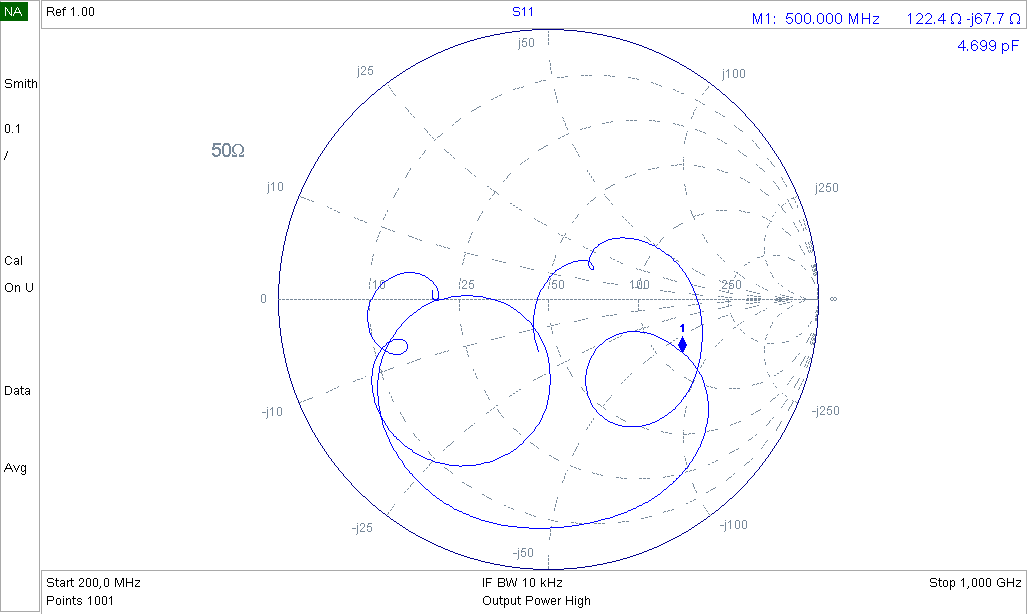
\includegraphics[width=9cm]{Images/impRFvieja.png}
		\caption{Impedancia del puerto RF.}
		\label{impedancia1fran}
	\end{figure}
	
	\indent En la Figura \ref{impedancia2fran} se muestran los resultados que se obtienen de realizar el mismo procedimiento al puerto O del mixer. 
	Para $f_{LO}=800~MHz$, la impedancia del puerto es de 
	$14.83\Omega-j\cdot15.29\Omega$. Sin embargo a una frecuencia cercana se obtiene un comportamiento que se aproxima mejor al deseado de $50\Omega$, en $f=859.9~MHz$, la impedancia del puerto es de $51.5\Omega+j\cdot3.04\Omega$.
	
	\begin{figure}[!htb]
		\centering
		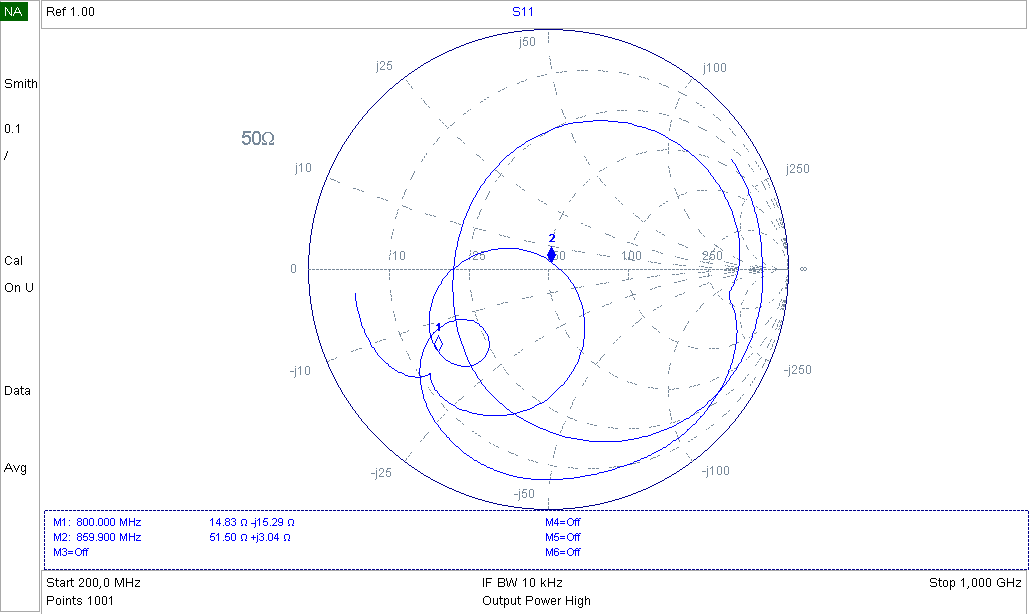
\includegraphics[width=9cm]{Images/impLOvieja.png}
		\caption{Impedancia del puerto LO.}
		\label{impedancia2fran}		
	\end{figure}

	\indent Finalmente se mide la impedancia del puerto IF. En la Figura \ref{impedancia3fran} se muestran los resultados obtenidos en el formato de la carta de Smith. Para $f_{IF}=800~MHz-500~MHz=300~MHz$ se obtiene una impedancias de $91.8\Omega+j\cdot75.3\Omega$
	habitualmente se desea tener.
	
	\begin{figure}[!htb]
		\centering
		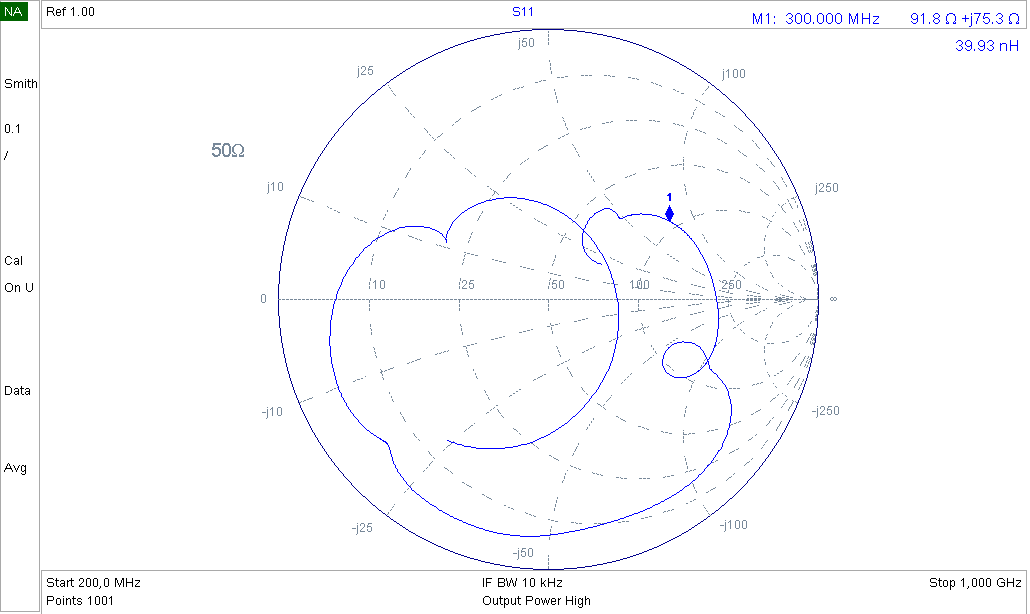
\includegraphics[width=9cm]{Images/impIFvieja.png}
		\caption{Impedancia del puerto IF.}
		\label{impedancia3fran}
	\end{figure}			
	Con respecto a las impedancias obtenidas anteriormente puede notarse que en este caso para todos los puertos la parte resistiva es mayor.
	
	\subsection{Aislación entre puertos}
	\indent Conectando el analizado de espectros PSA 6000 en el puerto de salida del mixer, el sintetizador de frecuencias N9310A al puerto de entrada y el puerto restante cargado con $50\Omega$ se calculan las aislaciones.
	
	\begin{itemize}
		\item Del puerto LO al puerto IF
	\end{itemize}
	
	\indent El sintetizador de frecuencias N9310A se conecta al puerto LO y se configura para tener una se\~nal de $0~dBm$ y $800~MHz$. Con el analizador de espectro conectado al puerto IF, se busca su amplitud en $f=800~MHz$ como se muestra en la Figura \ref{isolation1fran}. La amplitud obtenida es de $-35.64~dBm~\pm~1.5~dBm$ por lo tanto
	
	$$\textmd{Aislaci\'on}=0~dBm-(-35.64~dBm~\pm~1.5~dBm)=35.64~dBm~\pm~1.5~dBm$$
	
	\begin{figure}[!htb]
		\centering
		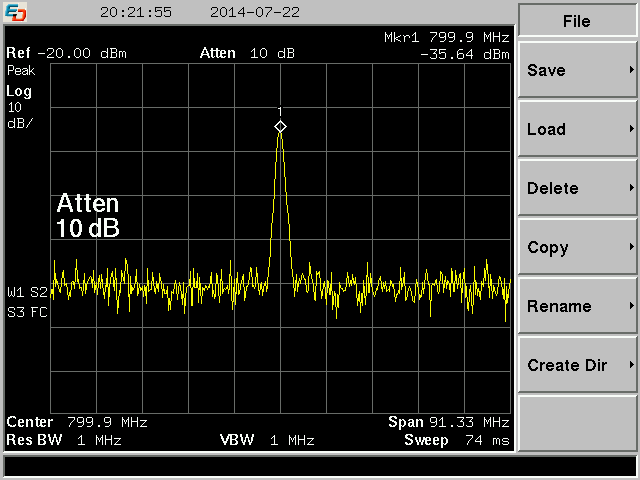
\includegraphics[width=10cm]{Images/SCREN531.png}
		\caption{Aislaci\'on entre los puertos LO y IF.}
		\label{isolation1fran}
	\end{figure}	
	
	\begin{itemize}
		\item Del puerto RF al puerto IF
	\end{itemize}
	
	\indent En este caso el sintetizador de frecuencias se conecta al puerto RF y se configura para tener una se\~nal de $0~dBm$ y $500~MHz$. El analizador se conecta al puerto IF, se obtiene su amplitud en $f=500~MHz$ como se muestra en la Figura \ref{isolation2fran}. La amplitud obtenida es de $-19.47~dBm~\pm~1.5~dBm$ por lo tanto
		
		$$\textmd{Aislaci\'on}=0~dBm-(-19.47~dBm~\pm~1.5~dBm)=19.47~dBm~\pm~1.5~dBm$$
	
	\begin{figure}[!htb]
		\centering
		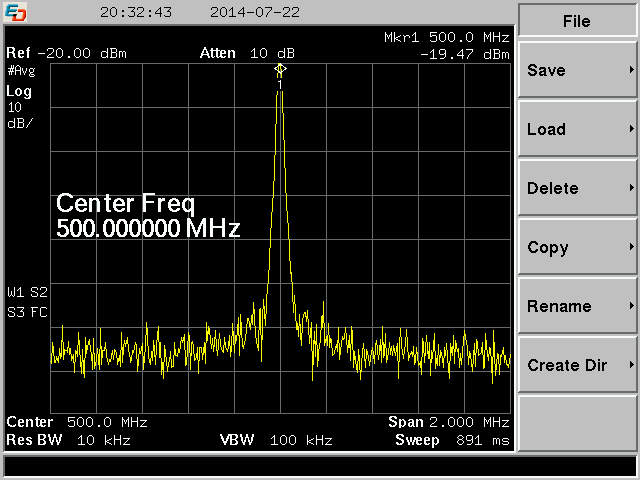
\includegraphics[width=10cm]{Images/SCREN534.png}
		\caption{Aislaci\'on entre los puertos RF y IF.}
		\label{isolation2fran}
	\end{figure}
	
	\begin{itemize}
		\item Del puerto LO al puerto RF
	\end{itemize}
	
	\indent Por \'ultimo se calcula la aislaci\'on del puerto LO al puerto RF. El sintetizador de frecuencias N9310A se conecta al puerto LO y se configura para tener una se\~nal de $0~dBm$ y $800~MHz$. El analizador se conecta al puerto RF, se obtiene su amplitud en $f=800~MHz$ como se muestra en la Figura \ref{isolation3fran}. La amplitud obtenida es de $-21.51~dBm~\pm~1.5~dBm$ por lo tanto
			
		$$\textmd{Aislaci\'on}=0~dBm-(-21.51~dBm~\pm~1.5~dBm)=21.51~dBm~\pm~1.5~dBm$$
	
	\begin{figure}[!htb]
		\centering
		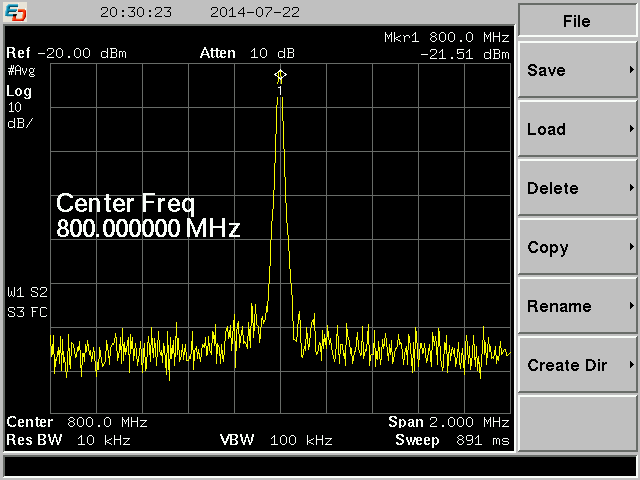
\includegraphics[width=10cm]{Images/SCREN533.png}
		\caption{Aislaci\'on entre los puertos LO y RF.}
		\label{isolation3fran}
	\end{figure}	
	
	En general las aislaciones obtenidas en este rango de frecuencias son mayores que las obtenidas previamente, en particular la de LO-IF y la de LO-RF, las cuales son las m\'as importantes ya que la se\~nal del puerto LO es la de mayor potencia.
\end{document}